\documentclass{beamer}
\usetheme{Madrid}
\usepackage{lmodern}
\usepackage{hyperref}
\usepackage{apacite}
\usepackage[utf8]{inputenc}
\usepackage[spanish]{babel}

\usepackage{xcolor}
\setbeamertemplate{background}{\tikz[overlay,remember picture]\node[opacity=0.2]at (current page.center){
\includegraphics[width=13cm]{KL.png}};}
\usepackage{tikz}
\usepackage{kantlipsum}

\setbeamercolor{normal text}{fg=black}

\begin{document}
\colorlet{beamer@blendedblue}{blue!46!green}
\setbeamercolor{normal text}{fg=black}

\setbeamercolor{frametitle}{fg=white, bg=blue!46!green}
\setbeamercolor*{title}{bg=blue!46!green, fg=white}

\setbeamercolor{section in toc}{fg=black}

\author[Juan C. Correa \textcolor{white}{(\url{https://correajc.com}})]{Juan C. Correa, Ph.D.}
\title[¿Qué es la Ciencia Abierta?]{¿Qué es la Ciencia Abierta?}
% \subtitle{TREME}
	%\subtitle{}
\institute[]{Fundación Universitaria Konrad Lorenz\\
	\color{blue}\Email  \href{mailto:juanc.correan@konradlorenz.edu.co}{juanc.correan@konradlorenz.edu.co}}
\pgfdeclareimage[height=0.5cm]{KL}{KL}
\logo{\pgfuseimage{KL}}
\setbeamertemplate{caption}[numbered]
\date[Bogotá, Mayo-2021]{Curso en: \textbf{T}ecnologías \textbf{R}eproducibles en la \textbf{E}nseñanza de la \textbf{M}etodología y la \textbf{E}stadística}

%\subject{}
\setbeamercolor{background canvas}{bg=white}
%\setbeamertemplate{navigation symbols}{}

\begin{frame}
	\titlepage
\end{frame}

\begin{frame}
\begin{block}{Objetivo del Curso}
\vspace{0.3cm}
Comprender la definición de ciencia abierta y su relación con Tecnologías Reproducibles para la Enseñanza de la Metodología y la Estadística.  
\end{block}
\end{frame}



\begin{frame}
\frametitle{Agenda} 
\tableofcontents
\end{frame}


% \begin{frame}
% \Huge
% \centering
% \textcolor{blue!46!green}{Elementos de Alfabetización Estadística en Psicología}
% \end{frame}

\section{¿Qué es la Ciencia Abierta?}
\begin{frame}{¿Qué es la Ciencia Abierta?}
\begin{figure}
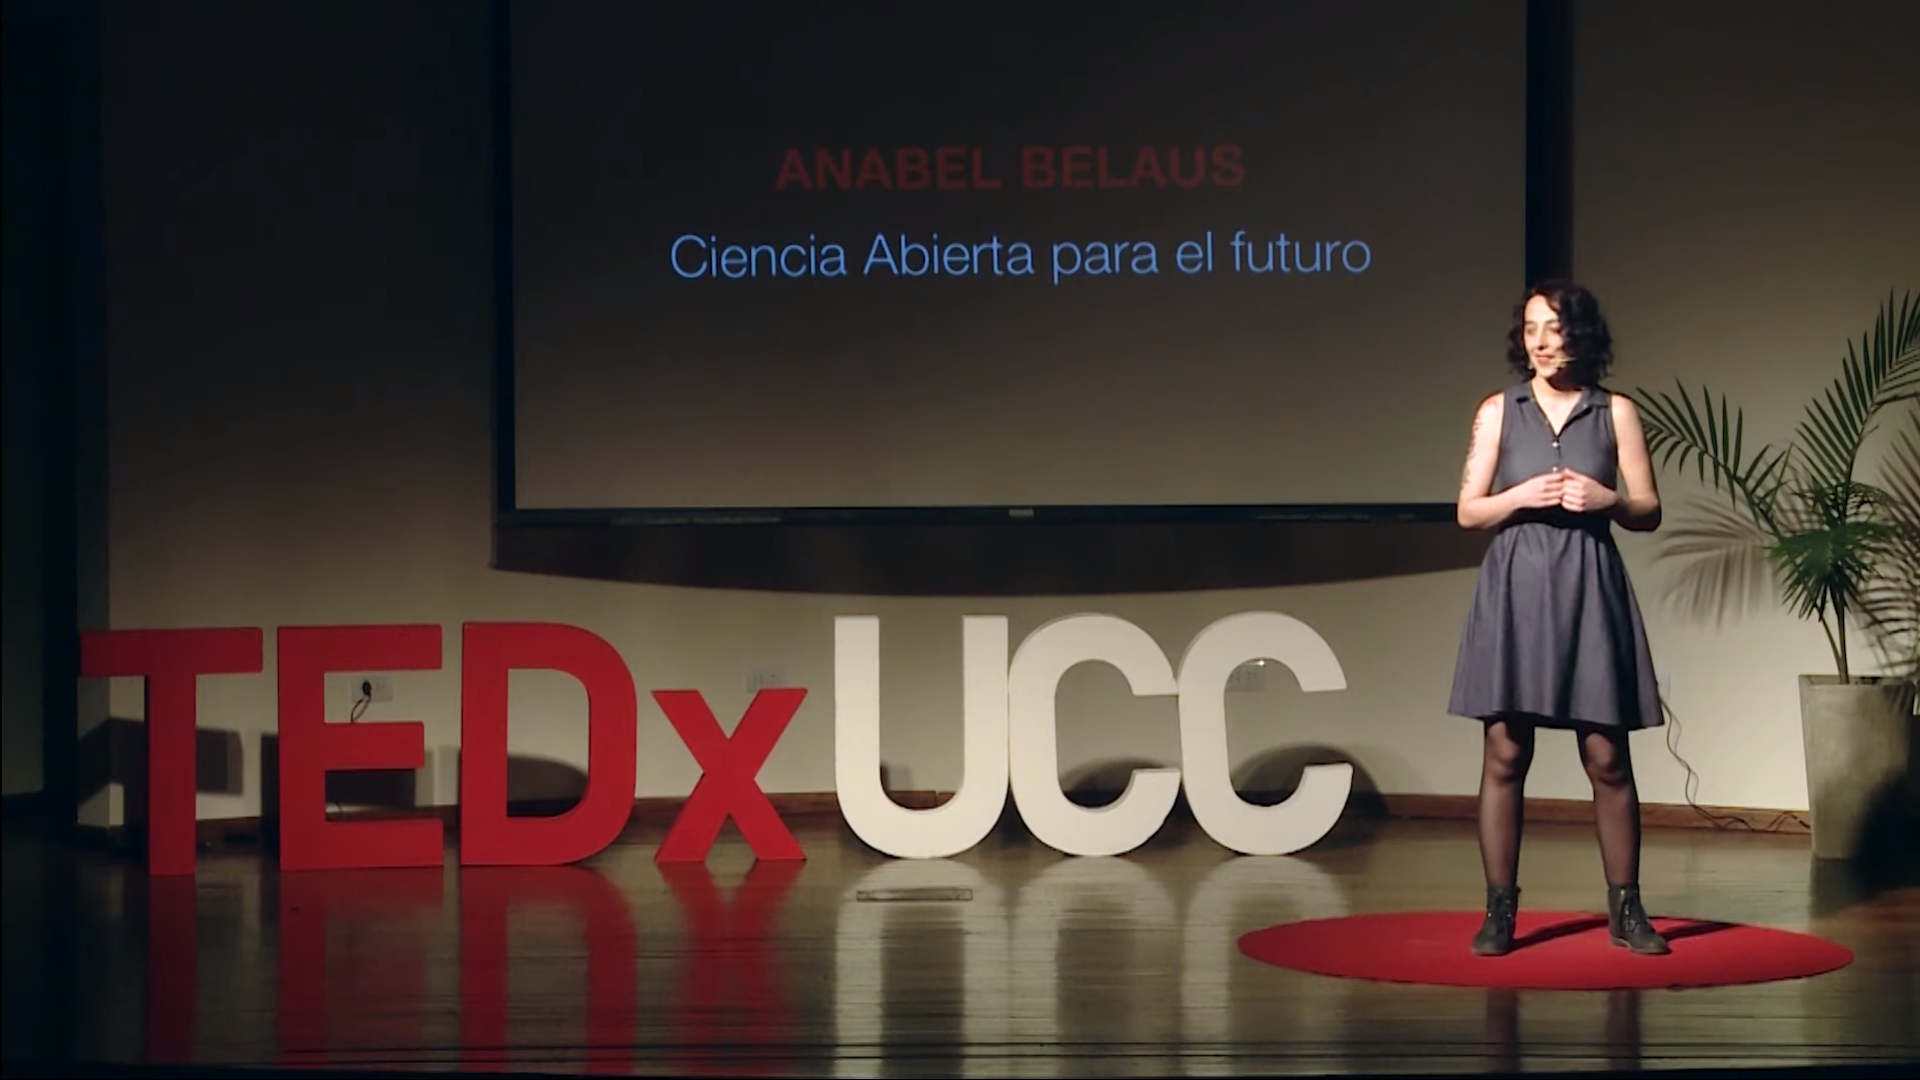
\includegraphics[width=.7\textwidth]{Anabela.png}
\end{figure}
\tiny
\textcolor{blue}{\url{https://www.ted.com/talks/anabel_belaus_ciencia_abierta_para_el_futuro}}
\end{frame}

\begin{frame}{¿Qué es la Ciencia Abierta?}
\large
¿Por qué la ciencia abierta plantea implicaciones para la enseñanza?
\begin{figure}
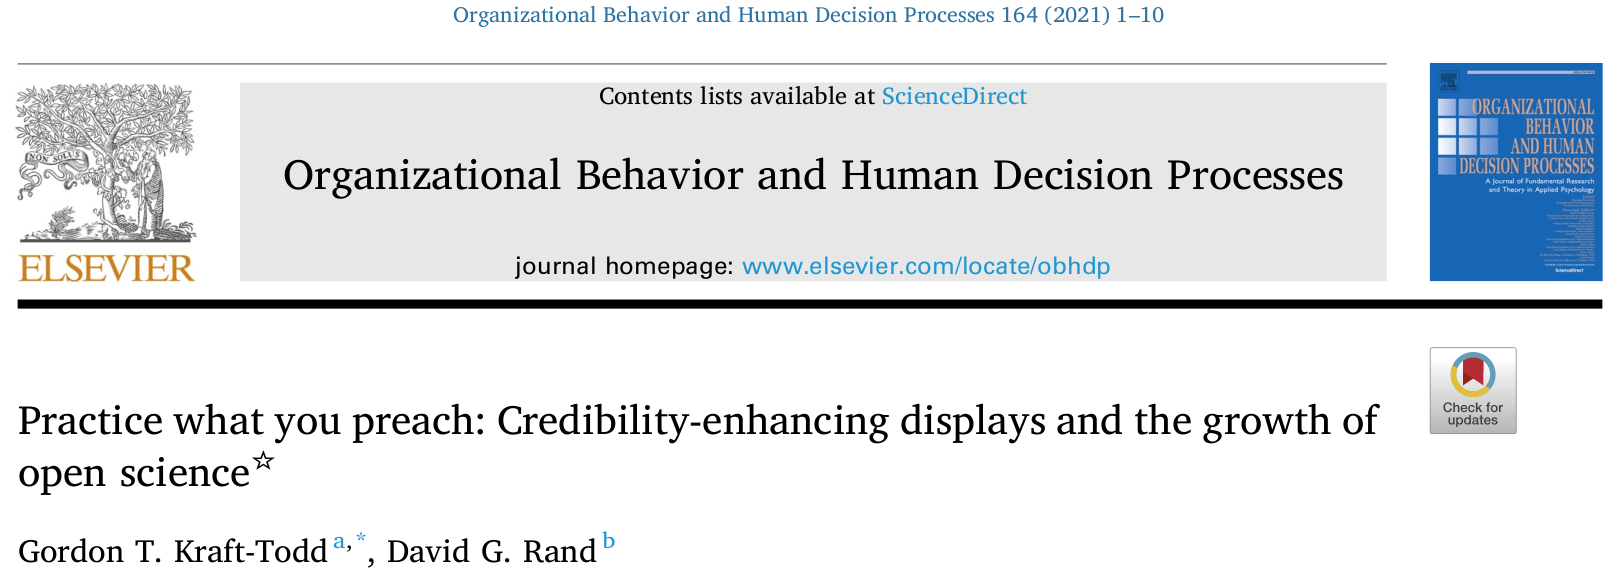
\includegraphics[width=.7\textwidth]{CA.png}
\end{figure}
\cite{Kraft2021}
\end{frame}

\begin{frame}{¿Qué es la Ciencia Abierta?}
\large
¿Por qué la ciencia abierta plantea implicaciones para la enseñanza?
\begin{figure}

\includegraphics[width=1\textwidth]{CAT.png}
\end{figure}
\cite{Sarafoglou2020}
\end{frame}

\begin{frame}{¿Qué es la Ciencia Abierta?}
\large
¿Por qué la ciencia abierta plantea implicaciones para la enseñanza?
\begin{figure}
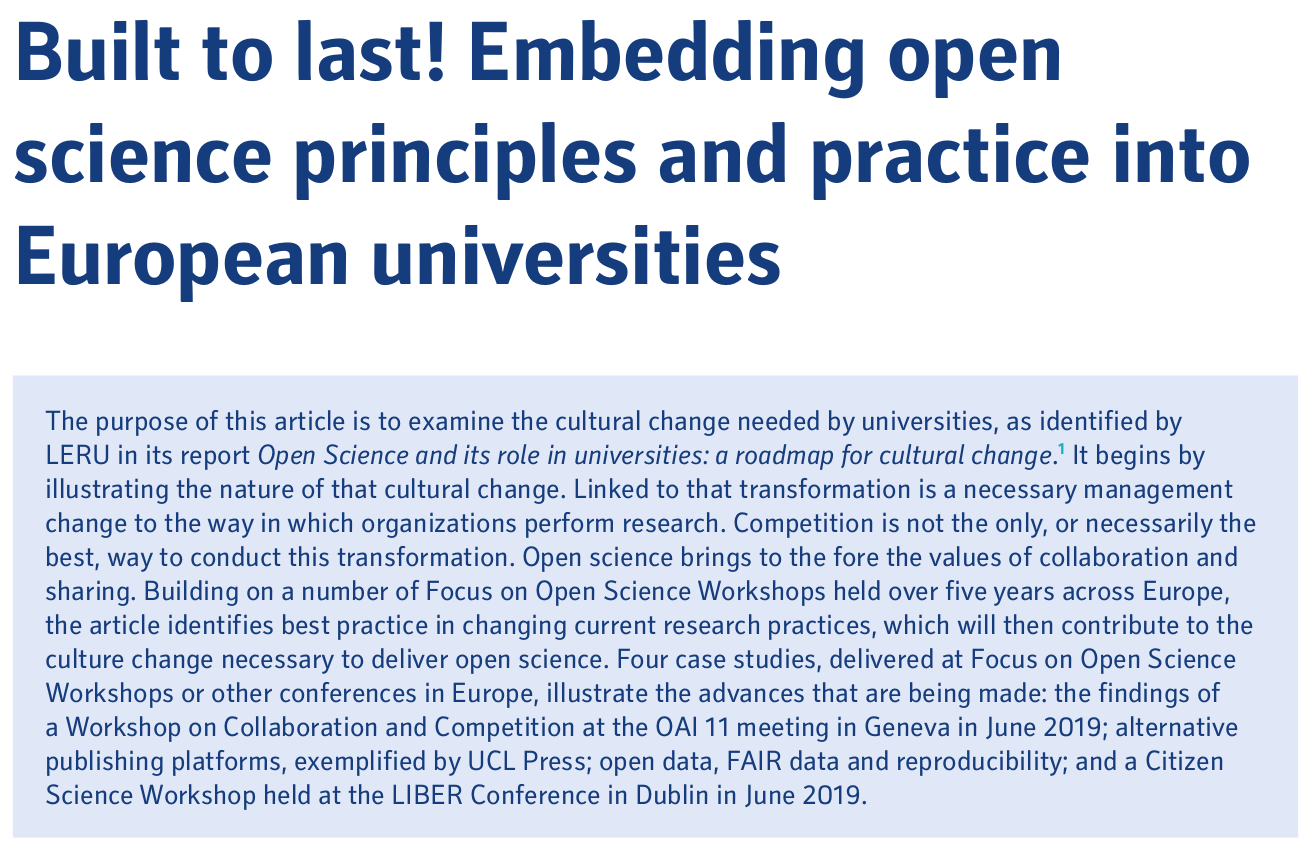
\includegraphics[width=.6\textwidth]{b2l.png}
\end{figure}
\cite{Ignat2021}
\end{frame}

\section{Algunas Implicaciones}
\begin{frame}{Algunas Implicaciones}
\begin{itemize}
    \item Cambio cultural de no compartir datos a compartirlos a la comunidad.
    \item Se aumenta la vida útil de los datos
    \item Se ofrece la posibilidad de reanalizar los datos y re-usarlos eficientemente (e.g., for meta-analyses)
    \item Se hace más probable la oportunidad de encontrar errores o fallas en los análisis estadísticos.
    \item Se comprende el origen de la crisis de replicabilidad y reproducibilidad en psicología.
    \item Se comprende cómo ha ocurrido el fraude científico.
    \item Se enriquece la formación hacia la investigación
\end{itemize}    
\end{frame}

\section{Caso de Estudio}
\begin{frame}{Caso de Estudio}
\begin{figure}
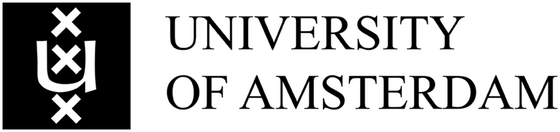
\includegraphics[width=.8\textwidth]{uA.png}
\end{figure}
Curso titulado ``Buenas Prácticas de Investigación'' adaptado a Maestría en Psicología.\\
Duración: 7 semanas, 14 horas de clases. Año académico 2018-2019.\\
Quizzes cada dos semanas sobre revisión de literatura, calidad presentaciones orales cortas, y asignaciones dentro de clases.\\
42 estudiantes de maestría en psicología.
\end{frame}

\section{Consideraciones Docentes}
\begin{frame}{Consideraciones docentes}
\begin{figure}
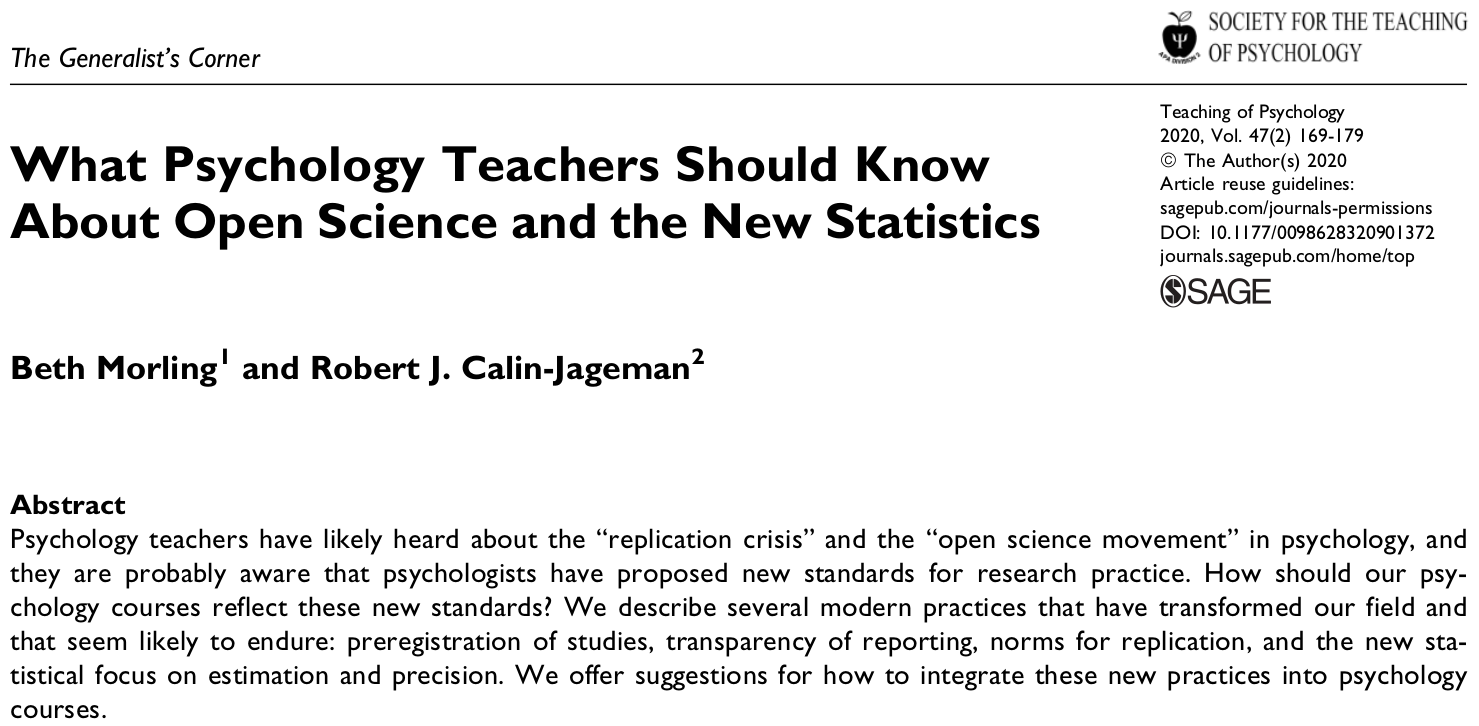
\includegraphics[width=1\textwidth]{Morling.png}
\end{figure}
\cite{Morling2020}
\end{frame}

\begin{frame}{Consideraciones Docentes}
\begin{figure}
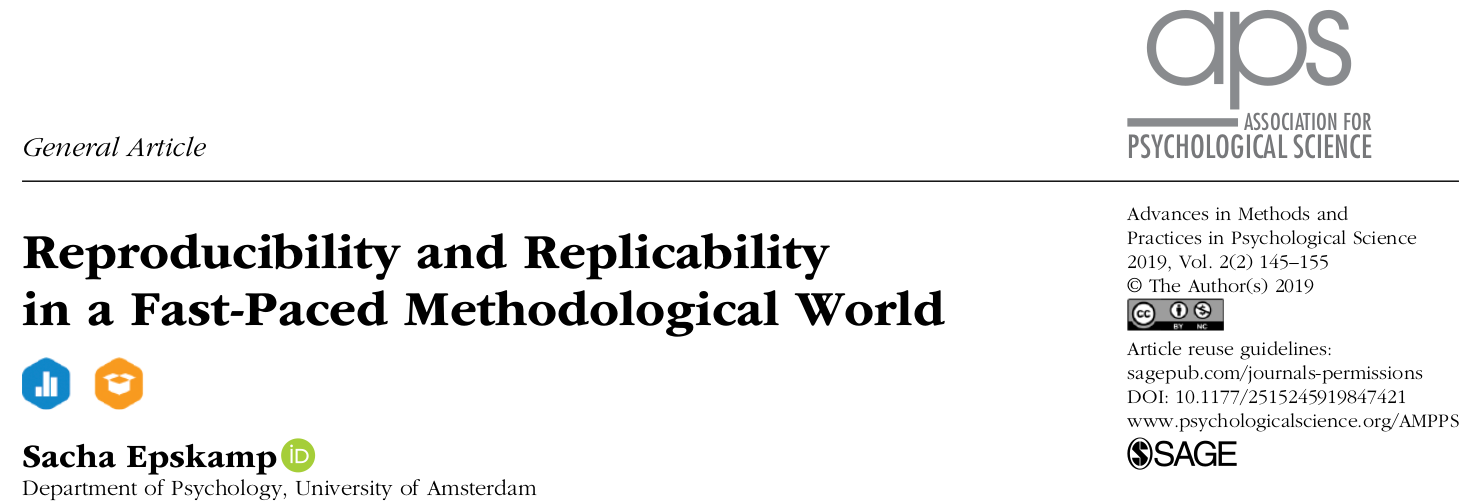
\includegraphics[width=1\textwidth]{Epskamp.png}
\end{figure}
\cite{Epskamp2019}
\end{frame}

\section{Ejercicio}
\begin{frame}{Ejercicio}
Se formarán dos grupos. Un grupo estudiará las consideraciones docentes planteadas en el paper de \citeauthor{Morling2020} \citeyear{Morling2020} y el otro grupo hará lo propio con el paper de \citeauthor{Epskamp2019} \citeyear{Epskamp2019}. Luego, cada grupo hará una presentación oral que sintetice las consideraciones docentes.
\end{frame}

\begin{frame}[allowframebreaks]{Referencias}
\tiny
\bibliographystyle{apacite}
\bibliography{refs} 
\end{frame}


\end{document}